\documentclass[a4paper, 11pt]{article}

\setcounter{tocdepth}{3}
\setcounter{secnumdepth}{3}

\usepackage{comment} % enables the use of multi-line comments (\ifx \fi) 
\usepackage{lipsum} %This package just generates Lorem Ipsum filler text. 
\usepackage{fullpage} % changes the margin
\usepackage[utf8]{inputenc}
\usepackage{gensymb}
\usepackage{graphicx}
\usepackage{booktabs}% http://ctan.org/pkg/booktabs
\usepackage{makecell}
\usepackage{tabularx}
\usepackage[table]{xcolor}
\usepackage{array}
\usepackage{wrapfig}
\usepackage{subcaption}
\usepackage{csquotes}
\usepackage{lscape}
\usepackage{afterpage}
\usepackage{geometry}
\usepackage{listings}
\usepackage{chngcntr}
\usepackage{multicol}

\counterwithin{figure}{section}

\geometry{a4paper, margin=1in}
\renewcommand{\figurename}{Abb.}
\renewcommand{\tablename}{Tabelle}
\newcommand{\code}[1]{\texttt{#1}}

\renewcommand*{\thead}[1]{\bfseries #1}

\renewcommand{\contentsname}{Inhalt}
\renewcommand{\listfigurename}{Abbildungsverzeichnis}


\begin{document}
	
\title{Zusammenfassung Future IT-Infrastructure FS2018}
\author{Alex Neher}
\maketitle

\tableofcontents
\newpage
\listoffigures
\newpage

\graphicspath{{./Pictures/}}

\section{Netzwerk-Aspekte}
\subsection{VPN}
Ein VPN (Virtual Private Network) erlaubt es einem Benutzer, sich in ein Netzwerk 'einzuklinken', selbst wenn er physisch nicht am Standort des Netzwerks ist.

\subsubsection{Szenarien}
Es gibt verschiedenste Szenarien, in welchen ein VPN nützlich oder vonnöten ist. Einige davon sind z.B:
\begin{description}
	\item [Remote Access: ] Management eines Kundennetzwerks vom (Home-)Office aus, Zugriff auf HSLU-Ressourcen von zuhause. US-Netflix in der Schweiz schauen
	\item[Site-to-Site VPN: ] Verbindung zweier Netzwerke über einen verschlüsselten Tunnel. Von der Azure-Cloud ins EnterpriseLab, Verbindung zwischen zwei fixen IPs.
\end{description}

\subsubsection{Technologien}
Es gibt verschiedene Technologien, wie ein VPN aufgebaut sind. die zwei wichtigsten sind:

\begin{description}
	\item[SSL-VPN] Wird vor allem für \textbf{Remote Access} verwendet, da es mit einem relativ einfachen Setup verbunden ist. SSL-VPN läuft ausschliesslich über \textbf{Port 443 (HTTPS)}
	\item[IPSec-VPN] Dieses Protokoll wurde ursprünglich exklusiv für IPv6 entwickelt, ist nun aber auch auf IPv4 portiert worden. Es kann, wie das SSL-VPN ebenfalls für Remote Access eingerichtet werden, ist jedoch auch nützlich für Site-to-Site VPNs. IPSec-VPN wird als \textbf{wichtigstes VPN-Protokoll} heutzutage angeschaut.
\end{description}

\noindent Des weiteren gibt es noch diese zwei, veralteten und unsicheren Protokolle, die jedoch immer noch eingesetzt werden.

\begin{description}
	\item[PPTP (Point-to-Point-Tunneling Protocol): ] Basiert auf PPP \footnote{Point-to-Pont-Protocol}, ist jedoch veraltet und unsicher.
	\item[L2TP (Layer 2 Tunneling Protocol): ] Ist unverschlüsselt und vertraut darauf, dass wichtige Daten verschlüsselt werden, bevor sie getunnelt werden. Dementsprechend veraltet und unsicher.
\end{description}

\newpage

\subsubsection{IPSec}

\begin{wrapfigure}[13]{L}{0.55\textwidth}
	\centering
	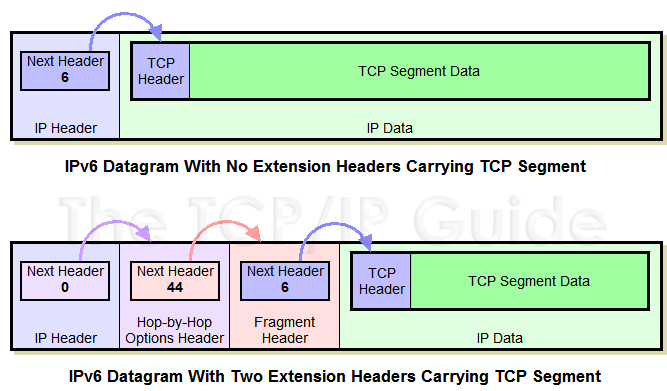
\includegraphics[keepaspectratio=true,height=10\baselineskip]{ipv6header.png}
	\caption{IPv6 unterstützt optionale Headers, die zwischen Payload und Header eingeschoben werden.}
	\label{fig:ipv6header}
\end{wrapfigure}


Da IPSec ursprünglich für IPv6 entwickelt wurde, unterstützt es dessen Konzept der \textbf{Header Extensions} (Abbildung \ref{fig:ipv6header}). IPv4 unterstützt jedoch \textit{keine} Header-Extensions! Bei IPv4 werden diese IPSec-Header einfach zwischen dem IP-Header und dem TCP/UDP-Header eingefügt.

\vspace{10px}

\noindent IPSec unterstützt die Verwendung des \textbf{AH} und/oder \textbf{ESP-Headers}.

\begin{description}
	\item[AH (Authentication Header): ] Die Authentizität des Datenursprungs ist sichergestellt.
	\item[ESP (Encapsulating Security Payload): ] Die Daten sind verschlüsselt
\end{description}

Die eingefügten Header beinhalten eingentlich nur eine \textbf{Sequenznummer} und einen \textbf{Index auf eine SA} (Security Association). Zudem wird das gesamte Paket noch mit einem \textbf{Hashwert} versehen, was jedoch dank NAT zu Problemen kommen kann, da das NAT die Authentizitäts-Garantie des Authentication Headers versaut.

\paragraph{Security Association} \mbox{} \\
Jedes IPSec Endgerät kann \textbf{beliebig viele} SA speichern. Eine SA ist grundsätzlich nur eine \textbf{Datenstruktur}, die (unter anderem) folgende Felder Informationen enthält:

\begin{description}
	\item[Authentifationsverfahren: ] Modi und Schlüssel falls AH verwendet wird.
	\item[Verschlüsselungsverfahren: ] Modi und Schlüssel, falls ESP verwendet wird.
	\item[Lebensdauer der SA und Schlüssel: ] Wie oft muss der VPN-Tunnel wiederhergestellt werden.
	\item[IP-Adresse der End-Netzwerk Gateways]
\end{description}

\noindent Beim Verbindungsaufwand wird diese SA aufgebaut. Dazu wird das \textbf{ISAKMP (Internet Security Association Key Management Protocol)} verwendet. 

\paragraph{ISAKMP}\mbox{} \\
Das ISAKMP Protokoll besteht aus zwei Phasen:
\begin{description}
	\item[Phase 1: ] Ein \textbf{gemeinsamer Schlüssel} wird mit einem \textbf{erweiterten Diffie-Hellman-Verfahren} ausgehandelt (Bürgler lässt grüssen). Anschliessend werden die \textbf{Verschlüsselungs- und Hash-Protokolle ausgehandelt (nun in verschlüsselter Kommunikation)}. Dabei gibt es zwei verschiedene Modi: Im Main-Modus einigen sich beide Parteien auf die verwendeten Protokolle, während im Aggressiven Modus der Initiator 'seine' Protokolle vorgibt. Die Partner authentisieren sich via PSK, ihre Digitale Signatur, RSA oder El-Gamal.
	\item[Phase 2: ] Die SA wird nun aufgebaut und die weiteren Parameter für die IPSec-Verschlüsselung und den Tunnel werden ausgetauscht.
\end{description}

\newpage

\paragraph{Transport- vs. Tunnel-Mode}\mbox{} \\
\begin{wrapfigure}[16]{R}{0.6\textwidth}
	\centering
	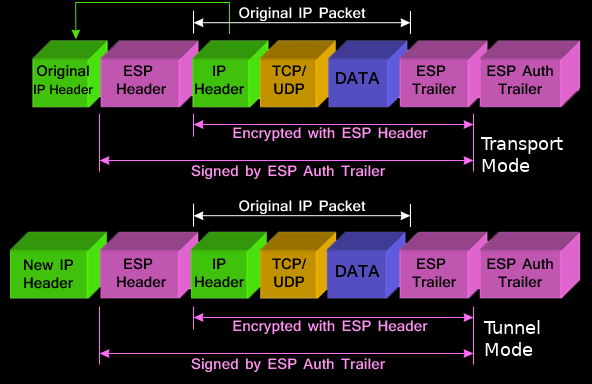
\includegraphics[keepaspectratio=true,height=12\baselineskip]{tunnelvstransport.png}
	\caption{Unterschied der Header zwischen dem Transport- und dem Tunnel-Mode}
	\label{fig:tunneltransport}
\end{wrapfigure}

Diese vorhin genannten weiteren Parameter sind z.B. ob der \textbf{Transport-} oder det \textbf{Tunnel-Modus} verwendet werden und ob \textbf{NAT-Traversal}\footnote{Ermöglicht es, das AH-NAT-Problem zu umgehen, indem die Pakete in UDP-Pakete encapsulated werden, die anschliessend über Port 4500 versendet werden..} erlaubt sein sollte.

Bei IPSec ist per Default der \textbf{Tunnel-Mode} eingestellt. In diesem Modus wird das \textbf{gesamte IP-Paket verschlüsselt}. IPSec nimmt es, verschlüsselt es, packt seinen IPSec Header davor und schickt es durch den Tunnel. Die allfälligen AH- und ESP-Header werden zwischen dem 'alten' IP-Header des zu verschlüsselnden Pakets und dem 'neuen' IP-Header des IPSec-Protokolls gepackt (Abbildung \ref{fig:tunneltransport} unten). 

Beim \textbf{Transport-Mode}, der hauptsächlich bei \textbf{End-to-End-Verbindungen)} wie z.B. Client zu Server eingesetzt wird, wird das IP-Paket durch \textbf{AH und/oder ESP-Header} verschlüsselt. Der IP-Header des Pakets wird beim Transport-Mode an den Anfang geschoben, gefolgt vom ESP (und evtl. AH-Header).

Transport-Mode wird meist mit einem anderen tunneling-Protokoll wie z.B. GRE gekoppelt. So wird der original Payload zuerst von GRP umschlossen, bevor IPSec das neue, umschlossene Paket durch den Tunnel schickt.

\paragraph{Verbindungsprobleme mit IPSec} \mbox{} \\
Es kann auch zu 'Show-Stopper' kommen beim Verbindungsaufbau mit IPSec, die verhindern, dass die Verbindung aufgebaut werden kann.

\begin{itemize}
	\item Der Initiator ist im Aggressiv-Mode und der Partner unterstützt die verlangten Protokolle oder den Aggressiv-Mode nicht (z.B. Android)
	\item Bei Remote Access VPN müssen IP-Adressen und weitere Informationen dynamisch übermittelst werden, die evtl. nicht untereinander kompatibel sind.
	\item Es gibt kein gemeinsames Set von Verschlüsselungs- oder Hash Algorithmen der beiden Seiten, bzw. die unterstützten Schlüssellängen sind nicht komptabiel.
\end{itemize}

In aller Regel sind Site-To-Site VPNs aber trotzdem möglich, solange die verwendeten Algorithmen bekannt und kompatibel sind.

\newpage

\subsection{WAN-Technologien}
\subsubsection{Definition}
WAN (Wide Area Network) sind \textbf{Netzwerk-Verbindungen} über \textbf{weite Distanzen}. Die Nutzen von WAN werden aufgeteilt in \textit{internet-basierte} und \textit{nicht-internet-basierte} Nutzen.
\vspace{10px}

\noindent  Internetbasierte Nutzen von WAN sind z.B. der Zugriff auf entfernte Ressoourcen über RDP oder Citrix, SSL-VPN oder Site-to-Site VPN via Internet.

\vspace{10px}

\noindent Nicht internet-basierte Nutzen von WAN sind z.B. Dark Fiber (Eine direkte Point-to-Point Verbindung zwischen zwei Standorten, die nicht am Internet hängt. Dark Fiber hat eine Reichweite von max 50km), LAN-Interconnect (Die Vereinigung zweier LANs über WAN), Private Lines oder Business VPN.

\subsubsection{Beurteilungskriterien}
Die Qualität von WAN-Verbindungen kann anhand verschiedener Kriterien gemessen werden.

\begin{description}
	\item[Geschwindigkeit: ] Kann die Geschwindigkeit, die der ISP verspricht auch garantiert werden?
	\item [Zuverlässigkeit: ] Wird die vereinbarte SLA zuverlässig eingehalten?
	\item[Kosten: ] Hat der Service ein vertretbares Kosten/Nutzen Verhältnis?
	\item[Redundanz: ] Garantiert der ISP eine Redundanz, falls eine Line unterbrochen wird?
	\item[Konfiguration \& Management: ] Welche Möglichkeiten bietet der ISP?
	\item[Provider/ISP: ] Welche Reputation hat der ISP? Wo ist er (vgl. Datenschutz), wie steht er wirtschaftlich da?
	\item[Sicherheit: ] Wie schützt der ISP die Verbindung?
\end{description}

\subsection{IPv6}
IPv6 (Internet Protocol version 6) ist der Nachfolger des heute am weitesten verbreiteten Internet Protokoll IPv4. IPv4 wurde in den Anfangsjahren des Internets entwickelt und ware nie dazu gedacht, solche Mengen von Geräten zu managen, die heute am Internet hängen. Deshalb bietet es nur eine sehr begrenzte Anzahl von öffentlichen IP-Adressen an (4.3 Milliarden öffentliche IPs vs. ca. 11.2 Milliarden Geräte in 2018 \footnote{Quelle: https://www.gartner.com/newsroom/id/3598917})). Durch 'verschwenderische' Vergabe dieser IP-Adressen in den 90er Jahren und strukturelle Begebenheiten des Protokolls (subnetting als Beispiel), sind diese IPs heutzutage so gut wie erschöpft.

IPv6, das bereits 1998(!!) vom IETF standardisiert wurde, besteht aus einer 128bit langen hexadezimal-Zeichenfolge. Dadurch bietet das Protokoll \textbf{340 Sextilionen ($340 * 10^{36} $) Adressen}. Ausserdem bietet es weitere, nützliche Features wie eingebautes QoS, Mobile IP oder erweiterte automatische Konfigurationen der Netzwerkschnittstellen.

\subsubsection{Adressierung}
Eine IPv6-Adresse ist ein 128bit langer hexadezimal-String. Er wird in 8 Blöcke zu je 16bit unterteilt, die mit einem Doppelpunkt voneinander getrennt werden.

Da 128bit hexadezimal-Strings ein bisschen komplizierter sind wie 32bit dezimal-Nummern, gibt es einige Vereinfachungen und Guidelines, die das Arbeiten mit IPv6 vereinfachen sollen:

\begin{itemize}
	\item Falls ein Block mit Nullen startet, können diese weggelassen werden. Somit wird die Adresse \code{2001:0db8:0000:08d3:0000:8a2e:0070:7344} zu \code{2001:db8:0:8d3:0:8a2e:70:7344}
	\item Falls ein ganzer Block (oder mehrere aufeinanderfolgende) ausschliesslich aus Nullen besteht, so kann er ganz weggelassen werden. Das darf jedoch nur \textit{einmal} pro Adresse gemacht werden. \code{2001:0db8:0000:08d3:0000:8a2e:0070:7344} kann also abgekürzt werden \\
	zu \code{2001:db8::8d3:0:8a2e:70:7344}.
	\item Die letzten 4 Bytes (32bit) einer Adresse dürfen auch in Dezimal angegeben werden. Dies ist vor allem hilfreich, wenn IPv4 Adressen zu IPv6 Adressen umgewandelt werden. So kann die IPv4 localhost Adresse \code{127.0.0.1}, die eigentlich zu \code{0:0:0:0:0:ffff:7f00:1} wird, kann zur besseren Verständlichkeit auch als \code{0:0:0:0:0:ffff:127.0.0.1} (oder abgekürzt \code{::ffff:127.0.0.1}) geschrieben werden.
\end{itemize}

IPv6 unterscheidet im Gegensatz zu IPv4 nicht zwischen public und private IP Adressen. Diese Tatsache eigentlich auch das NAT obsolet, dessen einzige Aufgabe es war, mehrere private IPs zu einer public IP zu mappen. Stattdessen wird eine Subnetzmaske definiert (standartmässig 64bit). Die ersten 64bit identifizeren das Netzwerk und die restlichen 64bit identifizieren den Host in diesem Netzwerk. \code{2001:0db8:85a3:08d3:1319:8a2e:0370:7347/64} bezeichnet also den Host/die NIC \code{1319:8a2e:0370:7347} im Netzwerk. Analog wie im IPv4 bezeichnet \code{2001:0db8:85a3:08d3::/64} das gesamte Netzwerk (wie \code{192.168.0.0} in IPv4). 

\vspace{10px}

\noindent IPv6 Adressen werden zwar nicht in private und public Adressen unterteilt, jedoch wird zwischen verschiedenen \textbf{Adressarten} unterschieden:

\begin{description}
	\item[Link Local Unicast: ] Jede NIC/jeder Host, der IPv6-enabled ist, erhält automatisch eine Link Local Adresse. Sie wird \textbf{automatisch erstellt} und ist einzigartig für jeden Host und wird von dessen MAC-Adresse abgeleitet. Dieser Adresstyp wird \textbf{nicht geroutet}, soll heissen diese Adresse ist nur vom lokalen Subnetz aus anpingbar. 
	
	Mithilfe der Link Local Adresse wird z.B. Neighbour-Discovery gemacht. Ebenfalls wird normalerweise die Link Local Adresse des Routers als Gateway angegeben. 
	\item[Unique Local Unicast: ] Wie bereits erwähnt, arbeitet IPv6 nicht mit private und public Adressen, was NAT eigentlich obsolet macht. Jedoch ist es manchmal trotzdem wünschenswert, ausschliesslich im lokalen Netz zu kommunizieren. Unique Local Unicasts werden \textbf{ausschliesslich im eigenen LAN geroutet}, nicht jedoch im Internet.
	\item[Global Unicast: ] Dies ist die öffentliche IP des Host. Sie wird \textbf{im LAN und im Internet geroutet}.
	\item[Multicast: ] Multicasts werden verschickt, wenn die Link Local Adresse eines Hosts noch nicht bekannt ist. Sie sind das \textbf{Equivalent des IPv4 Broadcasts}.
	\item[Site Local Unicast: ] Vorgänger des Unique Local Unicasts, veraltet.
\end{description}

\subsection{Software Defined Networks}
\subsubsection{Momentaner State-of-the-Art}
Momentan werden Netzwerke \textbf{statisch} aufgebaut. Es wird geplant, getestet und anschliessend aufgebaut. Jede Änderung unterliegt dem \textbf{Change-Management} und muss zuerst genehmigt werden. Dasselbe gilt für virtualisierte Netzwerke wie z.B. VMWare-Cluster etc.).

%TODO: SDN


\section{Identity Management}

\subsection{Geschichtliches}
Als der Übergang von standalone-Systemen zu vernetzten Rechnersystemen stattfand, mussten Rechner plötzlich Informationen von anderen Rechnern im gleichen Netzwerk abfragen (wie z.B. IP- oder MAC-Adressen). Zudem mussten Benutzer in der Lage sein, Informationen/Dateien von anderen Rechnern abrufen und bearbeiten zu können. 

In den 8er Jahren kam schlussendlich die Idee auf, eine weltweite Datenbank mit allen vernetzten Rechnern aufzusetzen:

\paragraph{X.500} sollte folgende Eigenschaften besitzen:
\begin{itemize}
	\item Verteilte Informationen
	\subitem Jede Firma verwaltet seine Informationen selbst
	\subitem Jede Firma bestimmt, welche Informationen veröffentlicht werden, also von aussen zugänglich sind.
	\subitem Alle Firmen können auf veröffentliche Informationen von anderen zugreifen.
	\item Hierarchische Struktur mit objektorientierter Ausrichtung
	\subitem Vorwiegend geographisch aufgebaut.
	\subitem Hierarchie ist den konkreten Bedürfnissen anpassbar.
	\subitem Berechtigungen und Sicherheit sind auf jeder Hierarchiestufe definierbar.
	\item Hohe Verfügbarkeit
	\subitem Verteilte Datenbanken 
	\subitem Replizierte Datenbestände
	\subitem Verteilte Administration
\end{itemize}

Es stellte sich jedoch recht schnell heraus, dass eine einzige, globale Datenbank schlicht und einfach zu komplex ist. Zudem wurde X.500 praktisch nicht genutzt, höchstens als E-Mail-Adressen-Verzeichnis. Daraus folgt, dass es fast keine Produkte auf dem Markt gab, was die gesamte Situation nicht wirklich verbesserte. Aufgrund dessen erachteten es Betriebssystem-Hersteller auch nicht für nötig, native Unterstützung dieser Norm zu implementieren. $\rightarrow$ \textbf{X.500 starb recht schnell wieder aus.}

\newpage

\subsection{Begriffe}
\begin{wrapfigure}[10]{R}{0.4\textwidth}
	\centering
	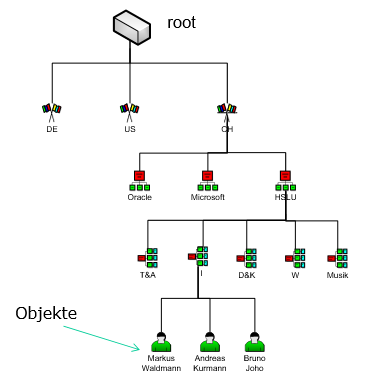
\includegraphics[keepaspectratio=true,height=10\baselineskip]{DIT.PNG}
	\caption{Beispiel eines DIT}
	\label{fig:dti}
\end{wrapfigure}
\paragraph{DIT - Directory Information Tree}\mbox{}\\
Der DIT wird verwendet, um Netzwerke darzustellen. Informationen werden hierarchisch dargestellt (siehe Abb. \ref{fig:dti} ). Im FAlle von X.500 war die Hierarchie Country (C) $\rightarrow$ Organization (O) $\rightarrow$ Organization Unit (OU). OUs halten weitere OUs oder Objekte, die mit einem Common Name adressiert werden. Am Beispiel von Abb. \ref{fig:dti} wäre ein Commmon Name 

\begin{lstlisting}
CN=Markus Waldmann, OU=Informatik, 
OU=I, O=HSLU, C=CH
\end{lstlisting}

\paragraph{DIB - Directory Information Base} \mbox{} \\
Die DIB ist eine Datenbank, in der alle Objekte des DIT gespeichert werden. Jedes Objekt hat verschiedene Attribute, die unterschiedliche Werte annehmen können.
\begin{figure}[htb]
	\centering
	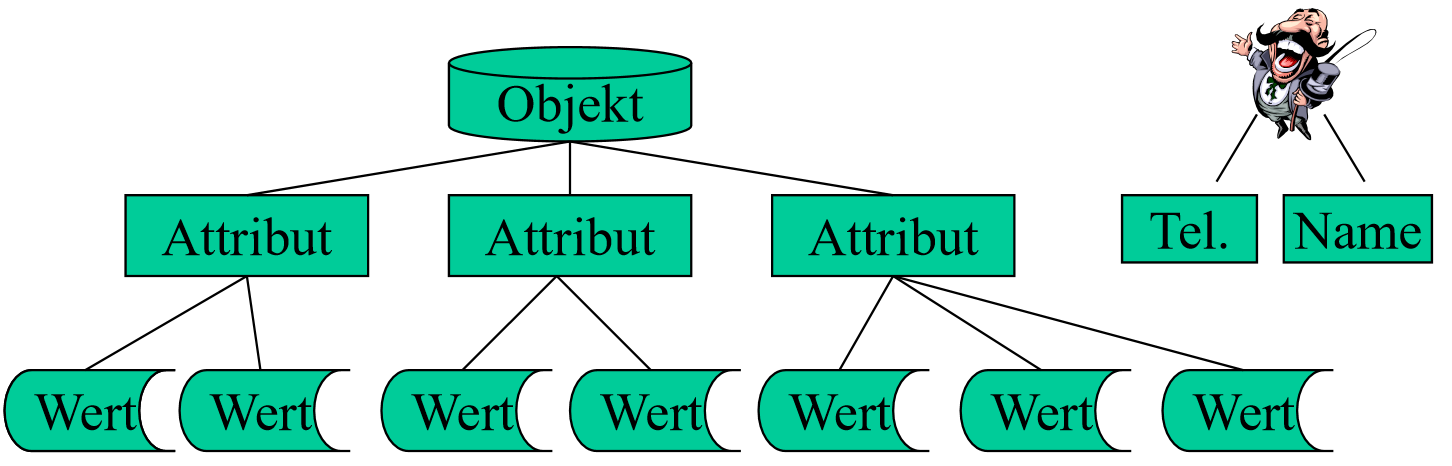
\includegraphics[keepaspectratio=true,height=10\baselineskip]{DIB.PNG}
\end{figure}

\paragraph{Schema}\mbox{}\\
eine Schema ist eine Ansammlung von Regeln, die Strukturen, Objekte und Datentypen beschreibt. Bei Bedarf kann ein Schema auch erweitert werden. Dank einem Schema ist eine Datenbank konsistent. 

Beispiel von Regeln sind:
\begin{itemize}
	\item Regeln zur Namenskonvention
	\item Regeln zur DIT-Struktur
	\subitem Wo können Objkete eingetragen werden?
	\subitem Welches sind zugelassene Super-Klassen?
	\item Regeln zu Objekt-Klassen
	\subitem Welhe Attribute kann und muss ein Objekt haben?
	\item Regeln zu Attributen
	\subitem Mögliche Datentpyen
	\subitem Mögliche Wertebereiche
\end{itemize}

\paragraph{ASN.1 - Abstract Syntax Notation}\mbox{}\\
Wie vorhin bereits erwähnt, besteht ein X.500 System ausschiesslich aus Objekten. Diese Objekte müssen irgendwie beschreiben werden. ASN.1 ist eine Sprache zur Beschreibung eines solchen Objekts.

\begin{lstlisting}
Name: Jan peter Schmidt
Geburtstag: 17.07.1957
...

PersonnelRecord ::= [APPLICATION 0] IMPLICIT SET {
Name, 
Titel [0] VisibleString, 
DateOfBirth [1] Date, 
(weitere Definitionen von Datentypen) 
} 
Name ::= [APPLICATION 1] IMPLICIT SEQUENCE {
Vorname VisibleString, 
Mittelname VisibleString, 
Nachname VisibleString 
} 
\end{lstlisting}

\paragraph{BER - Basic Encoding Rules}\mbox{}\\
BER basiert auf ASN.1 und übersetzt komplexe Daten in einen Datenstrom.

Aus
\begin{lstlisting}
Person   ::=  SET{
name     IA5String,
age      INTEGER
female   BOOLEAN
}

SET IA5String Maggie INTEGER 4 BOOLEAN TRUE
(Maggie ist eine 4 Jahre alte Frau)
\end{lstlisting}
wird
\begin{figure}[htb]
	\centering
	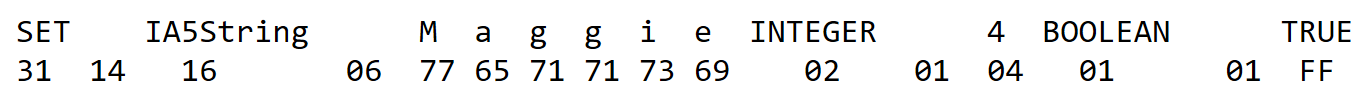
\includegraphics[keepaspectratio=true,height=2.5\baselineskip]{maggie.PNG}
\end{figure}

\newpage

\subsection{LDAP}
LDAP steht für \textit{Lightweight Directory Access Protocol} und ist prinzipiell nichts anderes wie X.500 mit dem TCP/IP Protokoll. Die Grundfunktionen von X.500 wurden beibehalten, jedoch lange nicht alle Funktionen.

Am Anfang wurden LDAP und X.500 parallel eingesetzt, indem ein Client übers Internet auf einen LDAP-Server zugreift, der die Anfrage schliesslich an einen X.500 Server weiterleitet (Abb. \ref{fig:ldapx500}).
\begin{figure}[htb]
	\centering
	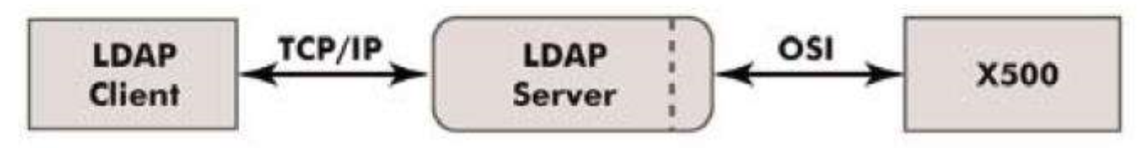
\includegraphics[keepaspectratio=true,height=2.5\baselineskip]{ldapx500.PNG}
	\caption{X.500 mit einem vorgeschalteten LDAP-Server}
	\label{fig:ldapx500}
\end{figure}

Später wurden die Funktionen, die vom X.500 nicht ins LDAP übernommen wurden schlicht nicht mehr benutzt, und der X.500 Service konnte immer mehr weggelassen werden, was heute immer noch der Standard ist (Abb. \ref{fig:ldaponly}).

\begin{figure}[htb]
	\centering
	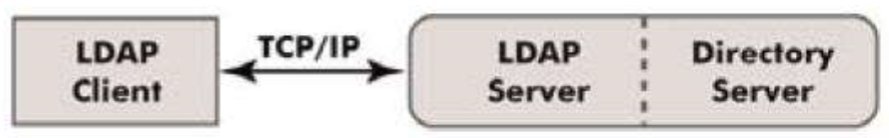
\includegraphics[keepaspectratio=true,height=2.5\baselineskip]{ldaponly.PNG}
	\caption{LDAP-Server ohne X.500 System dahinter}
	\label{fig:ldaponly}
\end{figure}

Zusätzlich wurden neue Features ausschliesslich in LDAP implementiert, wie z.b. Sicherheitsanforderungen, Erweiterbarkeit, Zeichensätze oder auch die Möglichkeit fremde LDAP Server zu referenzieren.

\vspace{10px}

\noindent Heute sind LDP Server Standard sowohl im UNIX wie auch im MS-Umfeld und immer mehr neue Anbieter (wie vCloud von VMWare) setzen auf LDAP. Jedoch ist die Interoperabilität zwischen einzelnen Produkten eher mangelhaft. Obwohl Interoperabilität zwischen verschiedenen Organisationen theoretisch möglich wäre, wird es praktisch nie eingesetzt.

\subsection{Microsoft Active Directory}
MS AD ist ein zentraler Ort für alle möglichen IT-Infrastruktur-Informationen wie
\begin{itemize}
	\item Benutzerverwaltung
	\item File Sharing und Berechtigungen
	\item Drucker
	\item Digitale Zertifikate
	\item Mail- und Fax-Adressen
	\item Kontakte
	\item Workstation- und Server-Konfiguration
\end{itemize}

Dank dem AD müssen Applikationen nicht mehr einzeln auf 500 Workstations installiert und konfiguriert werden, sondern das kann alles zentral über sog. Group Policies erreicht werden. Das AD funktioniert auch als globales E-Mail Adressenverzeichnis.

\newpage

\noindent MS AD unterstützt Standards wie LDAP, Kerberos (Authentifizierung), DNS, DHCP und RADIUS. Ausserdem bietet es ein ausgereiftes Administrationsmodell, welches eine Netzwerkweite Administration oder die auch die Delegation von einzelnen administrativen Aufgaben unterstützt. Das Active Directory kann auch in grossen Organisationen eingesetzt werden, da es auch mit mehreren Millionen Objekten problemlosläuft und dank einem organisationsweiten Schema werden auch Regeln für die Objekterstellung forciert.

\vspace{10px}

\noindent Objekte können auf verschiedene Arten angesprochen werden: 

\begin{description}
	\item[LDAP-Qualifizierter Name: ] CN=MWaldmann, OU=I, DC=HSLU, DC=CH
	\item[UNC/URL Notation: ] hslu.ch/I/MWaldmann
	\item[UPN Notation: ] MWaldmann.I@hslu.ch
	\item[GUID: ] tawaldma
	
	Die GUID ist insofern heikel, dass sie im gesamten AD gültig sind, das heisst "sekretariat" kann z.B. in einer grösseren Organisation mit verschiedenen Departementen nicht mehr verwendet werden, da der Name AD-weit eindeutig sein muss. $\rightarrow$ Eine AD-weite Namenskonvention muss definiert werden.
\end{description}

\subsection{Identity Management}
\blockquote{Entität = Etwas das existiert, etwas Seiendes.
	
	Identität = Völlige Gleichheit, Übereinstimmung in allen Merkmalen}

\blockquote{Eine digitale Identität ist die Teilmenge der Attribute einer Entität, welche diese Identität in einem bestimmten Kontext im Unterschied zu anderen Entitäten bestimmbar machen.

Eine Entität kann abhängig vom Kontext und den dadurch erforderlichen Attributen auch mehrere digitale Identitäten besitzen.}

\subsection{Laws of Identity}

\begin{enumerate}
	\item \textbf{User Control and Consent} \\
			Ich kann dem System, das meine Daten speichert vertrauen, indem ich selbst entscheiden kann, welche Identitäten und Daten ich wem preisgibt.
	\item \textbf{Minimal disclosuder for a constrained use}\\
			Daten werden nur auf einer "need-to-know"-Basis gesammelt und nur so lange behalten wie unbedingt nötig. Dies aufgrund dessen, dass je weniger Daten gespeichert werden, desto weniger Daten können gestohlen werden.
	\item \textbf{Justifiable parties}\\
			Mit wem werden welche Informationen geteilt?. Ich habe das Anrecht darauf zu wissen, wem meine Daten zu welchem Zweck zur Verfügung gestellt werden.
	\item \textbf{Directed Identification}\\
			Es muss unterschieden werden zwischen "omnidirektional" und "unidirektionalen" Identifikatoren. 
			
			Ein omnidirektionaler Identifikator identifiziert sich gegenüber jedem, der sich dafür interessiert wie z.B. die URL www.microsoft.com mit einem gültigen SSL Zertifikat. Jeder den es interessiert, kann überprüfen, ob diese URL tatsächlich das ist, für was es sich ausgibt: Eine URL der Microsoft Corporation. 
			
			Der unidirektionale Identifikator wiederum identifiziert sich ausschliesslich gegenüber der fragenden Partei. Angenommen, eine Website fragt mich nach meinem Alter, dann werden diese Daten ausschliesslich an diese Website weitergeleitet und nirgendwo anders hin. Wenn ich 5min später auf eine andere Website geht, so kennt diese mein Alter nicht.
	\item \textbf{Pluralism of Operators and Technologies}\\
			Es soll mehrere, verschiedene Identifikationssysteme geben.
			
			Es macht keinen Sinn, sich mit der AHV-Nummer beim Geschäfts-PC einloggen zu können. Denn der Staat hat Informationen über mich, die den Arbeitgeber vermutlich nichts angehen. Das heisst, für verschiedene Dinge sollten unterschiedliche Identifikationssysteme mit unterschiedlichen Features verwendet werden.
	\item \textbf{Human Integration}\\
			Die bisherigen Laws of Identity befassen sich hauptsächlich mit System-System oder auch Benutzer-System Interaktion. Diese Kanäle sind bereits recht gut gesichert. Was ist aber mit der Benutzer-Benutzer Interaktion? Wie kann ich sicherstellen, dass der nigerianische Prinz, der mir sein ganzes Geld vermachen will auch tatsächlich der ist, für den er sich ausgibt und kein Betrüger?
	\item \textbf{Consistent Experience Across Contexts}\\
			Wie bereits in Punkt 5 angesprochen muss es verschiedene Identifikationssysteme geben. Ich gebe auf dem E-Banking Portal nicht dieselben Informationen preis, die ich auf Facebook preisgebe. Es ist ein anderer Kontext und somit eine andere digitale Identität. Das Ziel ist es, diese Identitäten greifbar zu machen, z.B. mit einem Icon auf dem Desktop, das ich doppelklicken, bearbeiten oder auch löschen kann, wie es mir beliebt.
\end{enumerate}

\noindent Zusammengefasst (und auf Englisch) kann man die Laws of Identity folgendermassen zusammenfassen:

\blockquote[MSDN-Website für Laws of Identity]{Putting all the laws together, we can see that the request, selection, and proffering of identity information must be done such that the channel between the parties is safe. The user experience must also prevent ambiguity in the user's consent, and understanding of the parties involved and their proposed uses. These options need to be consistent and clear. Consistency across contexts is required for this to be done in a way that communicates unambiguously with the human system components.
	
As users, we need to see our various identities as part of an integrated world that nonetheless respects our need for independent contexts.}

\subsubsection{IAM in Firmen}
\begin{itemize}
	\item Applikationsspezifische Applikationsverwaltung
	\item ID-Daten in verschiedenen ID-Stores abgelegt
	\item Benutzer muss sich mehrere Passwörter merken
	\item Meist keine einheitlichen Security-Policies
	\item Keine durchgehenden Berechtigungsvergabe-Prozesse
	\item Manuelles Erzeugen/Löschen von Accounts
	\item Kein zentrales Access Management
	\item Viele grössere Organisationen haben zusammengeschusterte Lösungen
	\item IAM-Lösungen langen auf dem Vormarsch
\end{itemize}

\subsubsection{IAM im Internet}
\begin{itemize}
	\item Benutzer hat meist mehrere Identitäten
		\subitem Cloud
		\subitem Social Networks
		\subitem Shopping
		\subitem Online Games
		\subitem etc...
	\item Pro Identität nur ein Account möglich
		\subitem Wobei heute Login via FaceBook / Google vielerorts möglich ist
	\item Viele Benutzer greifen zu Notlösungen, um ihre Identitäten im Griff zu halten
		\subitem Überall gleiche Credentials
		\subitem Vergessene Credetials
		\subitem Passwörter aufschreiben
	\item Singe Sign On ist ein Bedürfnis
		\subitem Jedoch soll der Nutzer trotzdem noch die Kontrolle über seine Daten haben.
\end{itemize}

$\rightarrow$ Federated Identity Management

\subsubsection{Federated Identity Management}

\begin{wrapfigure}[16]{R}{0.55\textwidth}
	\centering
	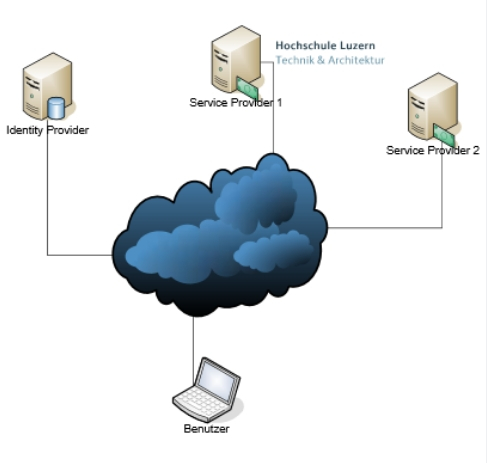
\includegraphics[keepaspectratio=true,height=15\baselineskip]{fim.jpg}
	\caption{Beispiel von Federated Identity Management}
	\label{fig:fim}
\end{wrapfigure}

Federated Identify Management ermöglicht es Benutzer, sich einmal bei einem Identity Provider einzuloggen. Alle anderen Services vertrauen anschliessend diesem Identity Provider, so dass sich der Benutzer nicht mehr bei ihnen einloggen muss ($\rightarrow$ Single Sign On).

Dank dem Federated Identity Management können nun system- und serviceübergreifend Authentifizierung und Autorisierung durchgeführt werden.

\vspace{10px}

\noindent Federated Identity Management ist essentiell für Cloud-Computing. Die meisten grösseren Cloud-Anbieter unterstützen bereits eine Art von Federated Identity Managent (SAML2 / ADFS von Microsoft, OpenID Connect, Shibboleth)

\paragraph{SAML 2}\mbox{}\\
SAML (Security Assertion markup Language) ist eine organisationsübergreifende Auszeichnungssprache für den Austausch von Authentifizierungs- und Autorisierungsinformationen,die auf XML basiert. 

Der Identity Provider ist die die Asserting Party (SAML Authority), welche die Identität eines Subjekts garantieren kann. Der Service Provider bietet einen Service an und vertraut dem Identity Provider.

\vspace{10px}

\noindent SAML 2.0 definiert sechs Request-Response Protokolle,die über XML-Schemata definiert werden. Es gibt zum Beispiel den Authentication Request (Ein Service verlangt die Authentifizierung des Benutzers) oder den Assertion Query and Request (Der Identity Provider bestätigt, dass der Benutzer irgendwann irgendwie authentifiziert wurde).

\vspace{10px}

\noindent Zudem werden über 6 sog. Bindings definiert, wie XML-Daten mit SAML übertragen werden wie z.B. über SOAP, HTTP Redirect oder HTTP POST.

\vspace{10px}

\noindent SAML 2.0 wird in den letzten paar Jahren vermehrt in markttauglichen Produkten eingesetzt, wie z.B dem MS ADFS (Active Directory Federation Service)

\begin{figure}[htb]
	\centering
	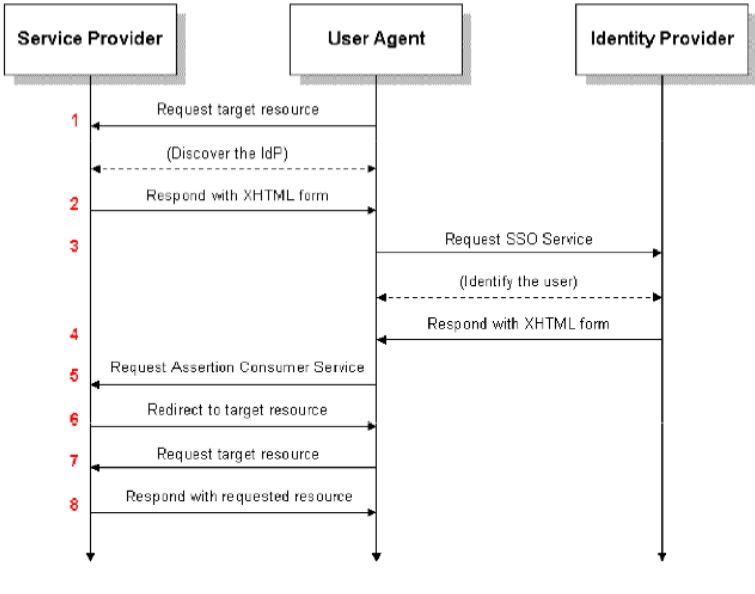
\includegraphics[keepaspectratio=true,height=20\baselineskip]{sso.jpg}
	\caption{Ablauf einer Authentisierung mit SSO Profil}
	\label{fig:sso}
\end{figure}

\paragraph{Shibboleth}\mbox{}\\
Shibboleth bietet ein Federated Identity Framework, welches vorwiegend im universitären Umfeld eingesetzt wird. Es ermöglicht Zugriffskontrolle, die auf einem Standard-Set von Attributen aufbaut, das jedoch bei Bedarf erweitert werden kann. Shibboleth ist zwar etwas Anderes als SAML 2.0, jedoch werden diese beiden Systeme immer kompatibler miteinander.

\vspace{10px}

\noindent Die Authentifizierung über Shibboleth läuft folgendermassen ab:

\begin{enumerate}
	\item Anfrage auf Ressource 
	\item Ressource redirected auf Discoveryservice (z.B. um auszuwählen zu welcher Hochschule ich gehöre) 
	\item User wählt die Hochschule aus 
	\item User wird zur Ressource redirected 
	\item Die Ressource leitet auf die Ressource der spezifischen Hochschule weiter 
	\item Dort muss sich der User mit den HS-Credentials anmelden 
	\item Der User wird auf die gewünschte Ressource weitergeleitet 
\end{enumerate}

\begin{figure}[htb]
	\centering
	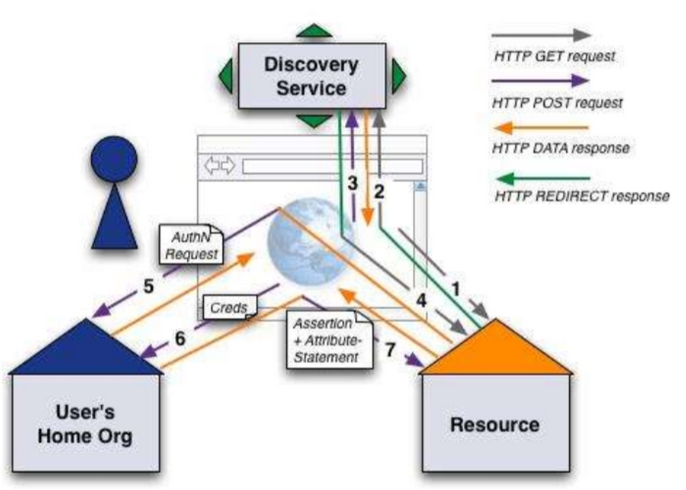
\includegraphics[keepaspectratio=true,height=15\baselineskip]{shibboleth.jpg}
	\caption{Ablauf der Authentifizierung über Shibboleth}
	\label{fig:shibboleth}
\end{figure}

\paragraph{OpenID}\mbox{}\\
OpenID ermöglicht die Authentifizierung über eine URL (z.B. portmal.clavid.com, www.clavid.com/portmann oder auch rportmann.startssl.com). Es gibt nur wenige Anbieter,die die Authentifizierung über OpenID zulassen und die Implementation hat noch einige Interoperabilitätsprobleme. Jedoch wäre dieser Standard Plattformunabhängig und stellt keinerlei Anforderungen an den Client.

\paragraph{OAuth}\mbox[]\\
OrganisationAuthentication ist ein open-source, tokenbasiertes Protokoll für die Autorisierung von APIs für sowohl Desktops wie auch Web- ud Mobile-Applikationen. Ein bekannteres Beispiel von OAuth ist die PKI-Karte. OAuth wird inzwischen von vielen grösseren Firmen intern verwendet und einige Cloud Anbieter haben es ebenfalls implementiert.

\paragraph{OpenID Conncect}\mbox{}\\
OpenID Connect gehört nicht zu OpenID sondern zu OAuth. Es fügt dem Autorisierungsprotokoll noch einen zusätzlichen Authentifizierungslayer hinzu. 

\paragraph{Digitale Signatur}\mbox{}\\
Zumindest in der Schweiz ist die digitale Signatur der handschriftlichen rechtlich gleichgestellt. Jedoch gibt es noch einige Probleme. So gibt es in der Schweiz zur drei zugelassene CAs, viele Signatursoftwares überprüfen nicht alle PDFs, sondern nur PDF-A Formate. Zudem müssen einige Geschäftsprozesse angepasst werden und die Archivierung muss regelkonform sein. Deshalb gibt es erst einige wenige tatsächliche Anwendung der digitalen Signatur hier.


\section{Cloud Resources}

Fallstudie

\newpage

\section{Evalutation von Cloud-Services}

Einige Aspekte die bei der Evaluation eines Cloud-Services berücksichtigt werden sollen:

\begin{multicols}{2}
	\begin{itemize}
		\item Kosten
		\item(Preis / Leistung)
		\item Funktionsumfang
		\item Vertragskonditionen (Wartung, Support, Ausstieg, usw.)
		\item Unterstützte Plattformen
		\item Sicherheit (Autorisierung, Datenschutz)
		\item Anpassungen des Service / Software
		\item Ruf der Firma
		\item Ausbau des RZ bezüglich Katastrophenschutz
		\item Wie oft gibt es einen neuen Release
		\item Einfachheit des Updateprozesses
		\item Performance
		\item Verfügbarkeit
		\item Skalierbarkei
		\item Wie viele andere Kunden gibt es
		\item Usability
	\end{itemize}
\end{multicols}

\subsection{Charakteristika eines Cloud-Services}

\begin{description}
	\item[On-Demand Self Service: ] Selbstzuweisung von Leistungen und Ressourcen aus der Cloud durch den Nutzer, die bei Bedarf bereitstehen.
	\item[Rapid Elasticity / Scalability: ] Funktionen und Ressourcen können schnell und dynamisch bereitgestellt werden, wenn möglich sogar automatisch. Aus Benutzersicht sind die Ressourcen "unlimitiert" und können jederzeit erweitert werden.
	\item[Broad Network Access: ] Die Services werden über ein internes oder externes Netzwerk zur Verfügung gestellt und können über standardisierte Schnittstellen auf unterschiedlichen Plattformen (wie Mobile oder Mac) genutzt werden.
	\item[Resource Pooling: ] Die Ressourcen des Providers werden nicht fest einem Benutzer zugeteilt, sondern alle verfügbaren Ressourcen werden in einem Pool gebündelt und dynamisch an die Benutzer vergeben, die es momentan brauchen.
	\item[Measured Service: ] Der Provider führt laufend QA	durch und versucht, seinen Dienst stetig zu verbessern.
\end{description}

\newpage

\subsection{Merkmale und Service/Deployment Modelle}

\begin{figure}[htb]
	\centering
	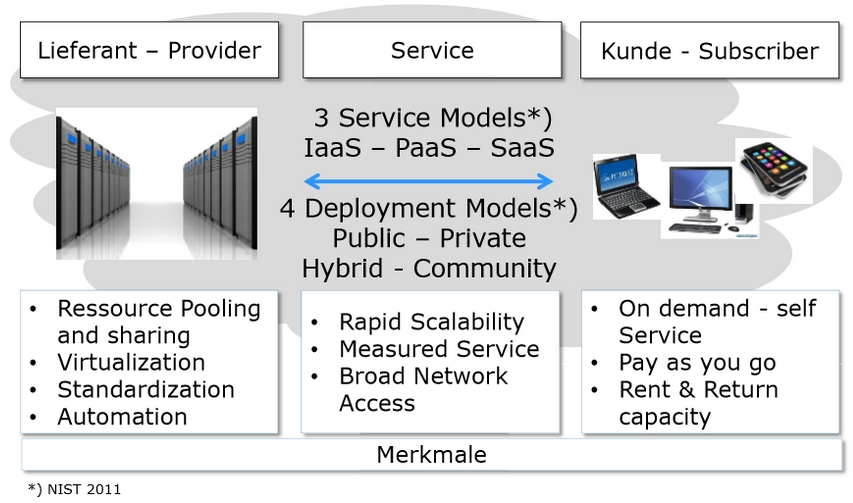
\includegraphics[keepaspectratio=true,height=15\baselineskip]{merkmale_cloud.jpg}
	\caption{Visualisierung der verschiedenen Service \& Deployment Modellen}
	\label{fig:merkmale_cloud}
\end{figure}
\begin{center}
\begin{tabular}{|l|p{10cm}|}
	\hline 
	\thead{Deployment Model} & \thead{In der Regel bedeutet das} \\ 
	\hline 
	Public Cloud & Für jedermann zugänglich. im Eigentum des Providers \\ 
	\hline 
	Community Cloud & Nur für bestimmte Gruppen von Benutzern oder Unternehmen zugänglich. Im Eigentum der Nutzer/eines Providers \\ 
	\hline 
	Private Cloud & Von einer einzigen Organisation genutzt. Kann im Eigentum dieser Organisation oder eines Providers sein.  \\ 
	\hline 
	Hybrid Cloud & Kombination aus verschiedenen Modellen. \\ 
	\hline 
\end{tabular} 
\captionof{table}{Unterscheidung verschiedener Cloud-Modelle}

\vspace{10px}


\begin{tabular}{|l|l|l|l|}
	\hline 
	\thead{Subkategorie} & \thead{Betreiber} & \thead{Standort} & \thead{Ressourcen-Sharing}\\ 
	\hline 
	Intern & Interne IT & Nutzer & Keines\\ 
	\hline 
	Outgesourced & Lieferant & Nutzer & Keines\\ 
	\hline 
	Hosted & Lieferant & Lieferant & Innerhalb des RZ und Netzwerks\\ 
	\hline 
	Virtual & Lieferant & Lieferant & Variabel\\ 
	\hline 
\end{tabular} 
\captionof{table}{Subkateorien von Privaten Clouds}
\end{center}

\subsection{ERP- und E-Business-System}
\paragraph{ERP System}\mbox{}\\
\begin{itemize}
	\item Aus mehreren Komponenten bestehendes integriertes Anwendungspaket
	
	(Integriert = Zieht Daten direkt aus der Datenbank, anstelle dass es selbst eine unterhält)
	\item Unterstützt die Abwicklung von Geschäftstransaktionen auf operativer Ebene
	\item Integriert in allen wesentlichen betrieblichen Funktionsbereichen
	\item Integration durch zentrale Datenbank
	\item Ermöglicht Abteilungsübergreifende Geschäftsprozesse
\end{itemize}

\paragraph{E-Business System}\mbox{}\\
Ein ERP-System mit einigen zusätzlichen Funktionen wie z.B.
\begin{itemize}
	\item Ermöglicht Betriebsübergreifende Prozesse
	\item Internet-Nutzung
	\item Zugang über Internet-Portale möglich
\end{itemize}

\subsection{Evaluationsverfahren}

\begin{figure}[htb]
	\centering
	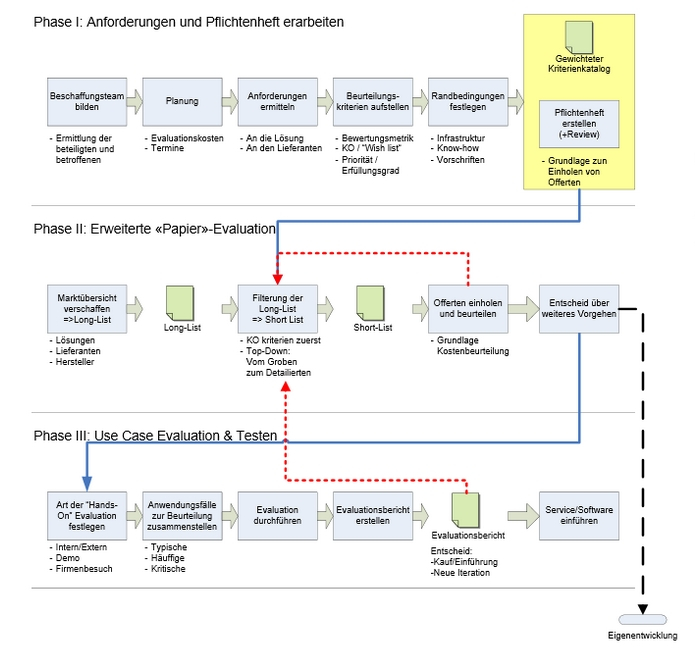
\includegraphics[keepaspectratio=true,height=25\baselineskip]{evaluation.jpg}
	\caption{Evaluationsvorgang bei der Auswahl eines Cloud-Services}
	\label{fig:eval}
\end{figure}

\subsubsection{Phase I - Anforderungen und Pflichtenheft erarbeiten}

\paragraph{Beschaffungsteam bilden}\mbox{}\\
Das Ziel dieses Arbeitsschrittes ist ziemlich selbsterklärend: Es soll ein Team gebildet werden, welches für die Evaluation und die Beschaffung des Services verantwortlich ist. Wichtig ist, dass die Endnutzer ebenfalls in den Prozess miteinbezogen werden.

Es sollten also Anforderungen für die gewünschten Personen definiert werden. Personen, die diese Anforderungen erfüllen können ins Team aufgenommen werden. Allenfalls muss noch ein externer Fachmann hinzugezogen werden.

Ebenfalls sollten alle involvierten Benutzer (also der Auftraggeber, die Steuerungsgruppe, der Projektleiter und die Endbenutzer) informiert werden.

\paragraph{Planung}\mbox{}\\
Das Ziel dieses Arbeitsschrittes ist es, den Scope, das Vorgehen und das Budget definiert zu haben. Es sollte ebenfalls bereits eine Deadline definiert sein. Schlussendlich sollte ein genehmigter Kosten- und Terminplan stehen.

Die Planung beinhaltet folgende Schritte:

\begin{enumerate}
	\item Ressourcen und Kapazitäten erfassen
	\item Evaluationsvorgang planen
	\item Kosten der Planungseinheiten abschätzen
	\item Planung abnehmen lassen
\end{enumerate}

\paragraph{Anforderungen ermitteln}\mbox{}\\
Bevor man sich für einen Service entscheiden kann, sollte man vorher noch abklären, zu was der denn überhaupt fähig sein müsste. Es muss also ein Anforderungskatalog erstellt werden, in dem die Anforderungen an den Service, dessen Dienstleister oder Lieferanten festgelegt werden.


\section{Platform Trends}

\section{Betriebliche Aspekte}

\end{document}